\chapter{Advanced Tasks}
\label{tasks}
This chapter is a selection of advanced tasks that can be done with \GigaMesh\!\!. Most of those tasks require several steps. In chapter \ref{example} the single steps will be accomplished in  brief examples, so skip the detailed description if you are already familiar with the program. The survey of the pulldown menu entries is given in chapter \ref{detdia} in great detail. 

Start the GUI-version of  \GigaMesh and open a 3D data file.

\section{Polishing the mesh}\label{GMOCFP}
Usually measured data is very nasty due to errors in the meshing of pointclouds. You have outliers, holes and twisted areas. In order to get rid of all these dirt in your mesh you
start by clicking on \texttt{Edit $\rightarrow$ Remove Unclean/Small}. You will be asked for the amount of small areas to be removed, the default is 10\% of the total surface. Now  the object gets cleaned prior to the fill holes algorithm. {\tt Remove Unclean/Small} is a compilation of several steps needed to optimize the mesh combined in one task. 

\begin{itemize}
\item remove {\em sticky faces} 
\item remove {\em non-manifold faces} 
\item remove {\em small areas} 
\item remove {\em solo vertices}
\item remove {\em singular vertices}
\end{itemize}

Sticky faces are faces using the same vertices and therefore stick together. Non-manifold faces occur when at least three faces share a common edge (see figure \ref{fig_manifold}). A small area is characterized by being not connected to other parts of the mesh and containing less than about 10\% of the total surface. A double cone is a face, that combines two parts of a surface at a single vertex. Solo vertices are  just single points without any edges connecting them to the mesh. Singular vertices happen when the borders of at least two holes meet in a vertex.

\begin{figure}[H]
 \centering
 \begin{tabular}{cc}
  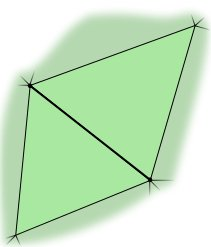
\includegraphics[width=3.0cm]{figs/manifold_egde} & 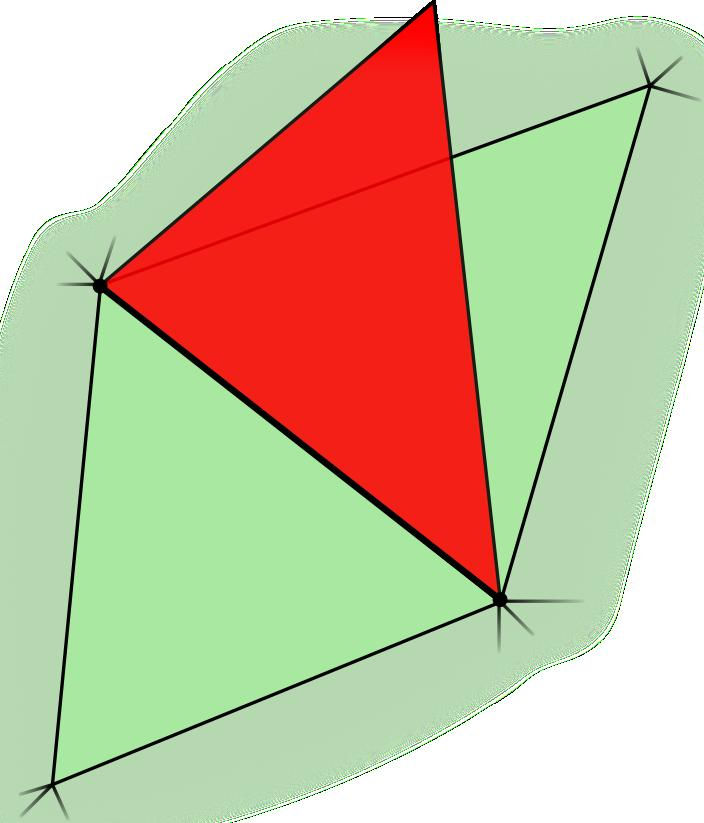
\includegraphics[width=3.0cm]{figs/manifold_egde_none}
 \end{tabular}
  \caption{a) manifold edge, b) non-manifold edge}\label{fig_manifold}
\end{figure}

The combined steps are to select e.g.~the solo vertices by \texttt{Select $\rightarrow$ Vertices $\rightarrow$ Solo} and then {\tt Edit $\rightarrow$  Remove SelVerts}. In the terminal the progress bar on each of the steps is reported.

Next go to \texttt{Analyze $\rightarrow$ Mesh Borders to Polylines} where all borders are selected as polygonal lines (short: polylines). The union of these lines form the boundary of the mesh. As result the boundary namely all these polylines are colored in light blue. In some cases these are only borders of tiny holes that can be immediately filled with  \texttt{Edit $\rightarrow$ Fill Holes (PSALM)}. There is no outer border of the mesh since the mesh is homeomorphic to a sphere e.g.~the head of a sculpture, or homeomorphic to a torus like e.g.~teapot. But in other cases the mesh has an outer border like just the face of a head or the front of a relief. Then the outer border does not belong to the category of holes to be filled. So you have to  \texttt{Select $\rightarrow$ Polyline Longest} which hopefully is this outer border and remove it from the list of polygonal lines (so-called polylines) to be filled.

Then the next step is to click on \texttt{Edit $\rightarrow$ Fill Holes (PSALM)}. Even a large number of holes get filled rather quickly and an info window informs about the number of holes which could be filled and those which are kept due to less information given or other errors reported in the terminal. After finishing the filled areas are colored in red to indicate where you do not have measured data and reliable color information. Finally you should get rid of all polylines.

Note that eventually this process has to be repeated several times since any time when removing vertices and when holes getting filled, new nasty areas might appear. So here again is the cycle to be repeated until the mesh is perfect:

\begin{enumerate}
\item  \texttt{Edit $\rightarrow$ Remove Unclean/Small} 
\item  \texttt{Analyze $\rightarrow$ Mesh Borders to Polylines}
\item  \texttt{Select $\rightarrow$ Polyline Longest}
\item  \texttt{Edit $\rightarrow$ Remove SelMPolylines}
\item  \texttt{Edit $\rightarrow$ Fill Holes (PSALM)}
\item  \texttt{Edit $\rightarrow$ Remove All Polylines}
\end{enumerate}

The mesh really is perfect, when no hole was filled and none was kept and the \texttt{Edit $\rightarrow$ Remove Unclean/Small} returns 0 Faces and 0 Vertices. Due to our naming convention you may save this file as an \GigaMesh {\bf GM} {\bf O}riented {\bf C}leaned {\bf F}illed {\bf P}erfect mesh and name it {\tt <filename>\_GMOCFP.ply}. If you miss out any of these steps, just leave out the according letter. You can just accomplish the specific task later.




\paragraph{Extend borders}
If holes cannot be filled as they are too large or too small they will be kept and the number of theses holes is shown in the finally popping up window. 
To make a hole easier to be filled or worked with it is sometimes necessary to extend its border and thereby making the hole larger. To do this go to \texttt{Select $\rightarrow$ Vertices - Border} and then click on \texttt{Edit $\rightarrow$ Remove - SelMVerts}.



\section{Visualize feature vectors}\label{wizard} 
Open the \texttt{<filename>\_r2.00\_n4\_v256.ply} file. 
Select the deepest cuneiform with a double click with the left mouse button. Correlated vertices are then visualized by clicking on \texttt{Functions $\rightarrow$ Feature Correlation to SelVert}. This may take some time. The default color map is {\tt Hot} but can be changed to anything you like best by selecting another map from the  \texttt{Colorramp}  e.g.~{\tt HSV} or {\tt Grayscale}. For other possibilities see section \ref{color}.


\section{Create a cross section with a cutting plane}
\GigaMesh features the possibility to create cutting planes. In order to get the proper outline of, e.g.~a vessel, this possibility sets a plane inside the vessel and ``cuts'' the object thereby showing its outline.

The first step is to \texttt{Select $\rightarrow$ Plane - 3 Points)} where the user will define a plane by three points: mark three points on the plane with (). The plane can be shown with \texttt{View $\rightarrow$ Mesh Plane}. In theory this plane is movable. Then calculate the distance to the plane. By selecting \texttt{Analyze $\rightarrow$ Iso Value - Set} the value for iso value should be set to 0. Then with \texttt{File $\rightarrow$ Export Screenshots (SVG + PNG) $\rightarrow$ Screenshot (SVG + PNG)} of the current view. This projects the polygonal lines to screenshots and calculates the outline.


\section{Unwrapping objects}\label{unwrap}
Objects being being approximately rotational symmetric can be unwrapped by specifying a sphere or a cone as auxiliary surface and projecting the object onto this surface prior to developing it to a plane. Choose {\tt Select  $\rightarrow$ Cone} and a user guiding sketch appears in the sidebar. It resembles a conical frustum and shows a red symmetry axis with a point $a$ that first has to be chosen by the user. To do so the object has to be positioned in such a way that you look down this symmetry axis of your object. Double click with the left mouse button to the position of this axis. The user guide sketch now indicates the second point $p_{r1}$ on a gray line perpendicular to the red axis and at the mantle of the cone. Select this point on the object by double click at a vertex of the surface. Now the user guide sketch indicates that the third point $p_{r2} $ has to be selected at the bottom of the cone. Selecting these three points results in a semitransparent red cone displayed together with the object. The red axis shows the symmetry axis and a green line indicates the split meridian. You may edit this prime meridian with {\tt Edit $\rightarrow$ Set Prime Meridian for Rollouts} and then move it around the cone with the left mouse button. You may also {\tt Edit $\rightarrow$ Cone - Set Cone Data} and change the radii manually. 

As long as {\tt Select $\rightarrow$ Cone} is still active, a double click will iterate the procedure of selecting those three points necessary for a cone description.

Finally {\tt Edit $\rightarrow$ Cone - Unroll Mesh} will execute the unwrapping. ATTENTION! This procedure is NOT reversible. To restart the unwrapping with another cone or sphere you have to reload the mesh from the data file.


\section{Fat cross or flat hexahedron}
In many cases you need a classic six-side view of the (visualized) model that is an orthogonal projection of the object onto the six sides of the bounding box. This can be done easily with this software. The first step to do this is to orient the 3D object either with the mouse or with the keyboard. Then hit \!\keystroke{F6} (this view will be saved as standard view) and save the file. Use the model ID you want. Next set the resolution with \texttt{Settings $\rightarrow$ Ortho Scale (Set DPI)}. After that go to \texttt{File  $\rightarrow$ Export Screenshots $\rightarrow$ Screenshot Views}. Since the main subject \GigaMesh has been developed for is visualization of cuneiform tablets, the popup menu entry for exporting  everything into a \LaTeX-file is called \texttt{Extra $\rightarrow$ Cuneiform Figure Latex Info}. In  step 7 of  section \ref{cuneiform} is a screenshot of the final view.


\section{Generating image stacks for videos or flashes}
\GigaMesh proposes the opportunity to create images that can be used for a flash video. The user can choose to create an image stack for a video moving the camera on a circular orbit around the object. The central axis of the orbit can be the horizontal axis of the view, the vertical axis of the view, a normal of a selected primitive, or the normal of a predefined plane.  This can be selected by  e.g~\texttt{File $\rightarrow$ Export Image Stack $\rightarrow$ 360° Circular Orbit Horizontal Axis}.

A flash video is similar to a video and additionally provides two interactions, firstly a rotation in two directions and secondly different states of the visualization can be shown, e.g.~the captured surface colors and the results of an MSII filtering. There exist several possibilities to create such image stacks. 
The  image stack for a flash moving the lightsource on a spherical orbit around the object can be chosen by \texttt{File $\rightarrow$ Export Image Stack $\rightarrow$ Spherical Stack Lightsource Orbiting}. Alternatively the camera is orbiting around the object. Therefore choose  \texttt{File $\rightarrow$ Export Image Stack $\rightarrow$ Spherical Stack Camera Orbiting}. By default, \texttt{Longitudinal} is selected, but you may change to \texttt{Altitudinal}. In order to separate the different visualizations, a state number can be given as a suffix for the filenames of the image stacks. Then these stacks can be processed into a flash object e.g.~with the {\em Garden Gnome Software} {\bf Object2VR}.

%First the user has to decide whether to rotate (a) the object  or (b) the lightsource during picture acquisition. If the user decides to move the object then the next choice is between (a1) horizontal and (a2) vertical axis movement. After these choices have been made in advance the pictures are generated very easily by clicking on \texttt{File $\rightarrow$ Spherical Images} (for the cases a1 and a2) or \texttt{File $\rightarrow$ Generate Spherical Images Light} (for case b). It is also possible to set the rotation axis for generating the stack of images.


%$\rightarrow$ ausführlicher, mehrere states (mit/ohne Textur), als tiff oder als png (Vorteil png: Flashes werden kleiner, Nachteil: bisher haben pngs transparenten Hintergrund $\Rightarrow$ schwarzer Hintergrund im Flash). 

%states: einmal anstarten, danach auf state number klicken, die um 1 höher setzen (von 0 auf 1) und alles nochmal durchlaufen lassen. Achtung! Namen müssen identisch sein.



\section{Usage of Object2VR with an image stack}
ATTENTION: This section describes how to generate a flash file using the software package {\bf Object2VR}.
\begin{enumerate}
\item Click on \texttt{select input} and choose \texttt{image sequence} as type
\item Set the path for the pictures in \texttt{file location}
\item Set the states right in \texttt{rows} and \texttt{columns} (e.g. spherical images requires 36 columns and 18 rows, states depends on how many have been done with GigaMesh. Attention: GigaMesh starts counting at 0).
\item Now the search string has to be given: 

%\[ '\texttt{filename}'+ \texttt{fill(column,5,0)} + '\_' + \texttt{fill(row,5,0)} + '\_' + \texttt{fill(state,2,0)} + '\texttt{.tiff}' \]
{\small \tt 'filename'+fill(column,5,0)+'\_'+fill(row,5,0)+'\_'+fill(state,2,0)+'.tiff'}

This command is for TIFF-files; for PNG-files just replace {\tt .tiff} by {\tt .png}.
\item Click on \texttt{test pattern}: here it is checked whether all files are found or not. If \texttt{all files found} then confirm with \texttt{ok}.
\item In \texttt{Viewing Parameters} select \texttt{modify} and set the initial position (this is optional). Hint: If \texttt{vertical images} has been selected in GigaMesh, the \texttt{horizontal} box has to be checked.
\item In output choose \texttt{Flash}, reduce the speed under \texttt{Autoplay} (appropriate: 0.05) and choose a skin (this can be the default or a self-made one).
\item If also needed for HTML, choose the tab \texttt{HTML} and check the box \texttt{enable html file}
\item Finally click on \texttt{ok} and answer the upcoming question with \texttt{yes}.
\end{enumerate}

\section{Sketch rendering}
\GigaMesh is able to render a 3D object in a sketch-like fashion. Sketch-rendering can be enabled by selecting \texttt{Colors $\rightarrow$ Sketch rendering}. With \texttt{Colors $\rightarrow$ Sketch rendering settings}, it is possible to customize the visualization. The sketch rendering consists of three different components: outlines, hatching/dithering and toon-shading. Each component can be enabled, disabled or customized under their respective tab.\\
The settings for \texttt{outline} are:
\begin{itemize}
\item \texttt{Enabled}: turns outlines on.
\item \texttt{Size}: determines the width of the outlines in screen-space pixels.
\item \texttt{Threshold}: threshold for the edge detection. Edges with a lower gradient than the threshold will be ignored.
\item \texttt{Color}: the color of the outlines.
\end{itemize}
The hatches or dithering can be customized in the following ways:
\begin{itemize}
\item \texttt{Enabled}: turns on hatching/dithering
\item \texttt{Size}: the size of the hatch-lines. This affects only the "Lines" and "Dots" styles
\item \texttt{Rotation}: angle of the hatch-lines in screen-space. This also affects only the styles "Lines" and "Dots"
\item \texttt{Color}: the color of the hatches
\item \texttt{Style}: a selection of different styles for shading. The following options are available:
\begin{itemize}
\item \texttt{Lines}: shade the object with a line-pattern
\item \texttt{Dots}: shade the object with a dot-pattern
\item \texttt{Random Dither}: shade the object with a pseudo-random dithering pattern
\item \texttt{Bayer Dither}: shade the object with a structured bayer-dithering pattern
\end{itemize}
\item \texttt{Light influence}: if enabled, the strength of the hatches is reduced with increasing light-intensity. Otherwise, the patterns are always rendered with full strength.
\end{itemize}
The toon-shading has the following options:
\begin{itemize}
\item \texttt{Enabled}: turns toon-shading on
\item \texttt{Diffuse Color $n$}: with these options, the diffuse color of the sketch can be changed. The number $n$ corresponds to the light intensity, where "0" means average light, positive numbers are brighter regions and negatives ones correspond to darker regions.
\item \texttt{Enable Specular}: if set, a specular highlight is shown.
\item \texttt{Specular Color}: the color of the specular highlight.
\item \texttt{Specular Size}: the size of the specular highlight.
\end{itemize}

\section{Transparency rendering}
Objects can be rendered semi-transparent by selecting \texttt{View $\rightarrow$ Transparency}. This option is only available if the GPU supports at least OpenGL 4.3, otherwise it is deactivated. The transparency-rendering has multiple settings which can be modified with \texttt{View $\rightarrow$ Transparency Settings}. The settings are divided into two main categories: \texttt{Transparency-Functions}, which influences how the opacity of an object is calculated, and \texttt{Buffer Types}, where different transparency-rendering implementations can be chosen. The following transparency-functions are available:
\begin{itemize}
\item \texttt{Vertex Color}:\\
This function takes the opacity-values directly from the vertex color of the mesh.
\item \texttt{Uniform}:\\
The uniform functions assigns one opacity-value to the whole mesh. The opacity-value can be changed with the \texttt{Alpha 1} slider.
\item \texttt{FuncVal}:\\
This function uses the normalized per-vertex function value as an interpolation-factor between \texttt{Alpha 1} and \texttt{Alpha 2}. The interpolation-factor is raised by the power of \texttt{Gamma}. Choosing a gamma-value less than one means, that \texttt{Alpha 1} is favored and values higher than one put more emphasis on \texttt{Alpha 2}. This can be used for a variety of effects. For example, one could store the geodesic distances to a vertex in the function-values. By choosing a low value for \texttt{Alpha 1}, and a high value for \texttt{Alpha 2}, the opacity increases by the distance to the reference vertex.
\item \texttt{LabelNr}:\\
\GigaMesh is able to assign labels to the vertices based on connected components. With this option it is possible to select one label. The vertices with the selected label will get the value of \texttt{Alpha 2} assigned, while every other one will receive the value of \texttt{Alpha 1}.
\item \texttt{Angle-Based}:\\
By selecting this option, transparency-values are assigned by the angle of the mesh-normals relative to the camera. Normals pointing directly towards or away from the camera take the value of \texttt{Alpha 1}, while the ones perpendicular get the value of \texttt{Alpha 2}. Values in between will be interpolated, using \texttt{Gamma}  as the exponent. The goal of this transparency-function is to hide obstructive areas, while keeping the contours intact.
\item \texttt{Normal-Variation}:\\
This function uses the variation of the normals to calculate the opacity. Areas with little to no variation will receive \texttt{Alpha 1}, while Areas with a high variation will receive \texttt{Alpha 2}. Values in between will be interpolated, using \texttt{Gamma} as exponent for the interpolation factor.
\end{itemize}
The user can choose three different implementations for transparency rendering. \texttt{Weighted Blend} is the fastest one with the lowest amount of memory consumption, but also the least accurate. This option should be chosen for low end graphics cards which have problems with the other options. However, the drawback is that transparent layers are very likely to appear to be too dark or too bright. \texttt{A Buffer} covers the high end of graphics card. The color-information is perfectly accurate, but also requires the most amount of memory and performance. \texttt{Atomic Loop} is the in-between option, which can also be tweaked for better quality or performance. \texttt{Atomic Loop} renders the closest $n$ layers accurately. The amount of layers can be selected with the \texttt{Num Layers} slider. Typically, values between ten and twenty should be sufficient. Choosing less will benefit performance, but drops of quality should become noticeable. Choosing more has generally little effect on quality, so it should be avoided to not waste performance. \texttt{Atomic Loop} has two ways to handle layers behind the first $n$ layers, which can be changed with the \texttt{Overflow Handling} drop-box. Those layers can either be discarded (\texttt{Discard}) for performance or to simply remove unimportant visual clutter, or blended together in the last layer (\texttt{Weighted Average}) for better quality.